%!TEX root = ../thesis.tex
\section{現況問題描述}
\label{c:ch3.2}
綜合上述,過往染整廠的做法大致是以工程師的經驗來決定製程參數的設定,以Datacolor MATCH所建議的染色配方做為打樣驗色及量產的配方。可是固定製程參數的設定會造成生產成本過高或是品質的不穩定,圖~\ref{fig:graph2}為染色配方和製程參數與染色表現間的反應曲面。假設當實驗結果出現如圖~\ref{fig:graph2}所呈現的極端曲面時,如果單純只考慮一個面向,染色配方或製程參數可能會出現一些問題。

圖~\ref{fig:graph2}的緃坐標為染色表現(設定為望大特性),可以看出平面A及平面C在固定各自的製程參數下,呈現出不同的染色表現。目前染整廠的做法只是固定製程參數設定,採用Datacolor MATCH所建議的染色配方,即是在平面A、C或是其他與A、C平行的平面,搜尋較佳染色配方。若固定某一染色配方時,製程參數的變動對於染色表現因子的影響用平面B的曲線來表達。由圖中可以看出選擇a點的製程參數有較佳的染色表現,固定a點的製程參數時,較佳的染色配方投射到平面C上的c點或d點,這兩點的染色表現明顯的比b點還要好。但如果只追求a點,則只要製程變數稍微改變,就會明顯的影響染色表現。相對的雖然b點沒有a點表現好,但由曲線可以觀察出即使製程變數稍微改變,染色表現依然不會降低太多,故可能選擇b點的方案是較為穩健的。
\begin{figure} 
\centering
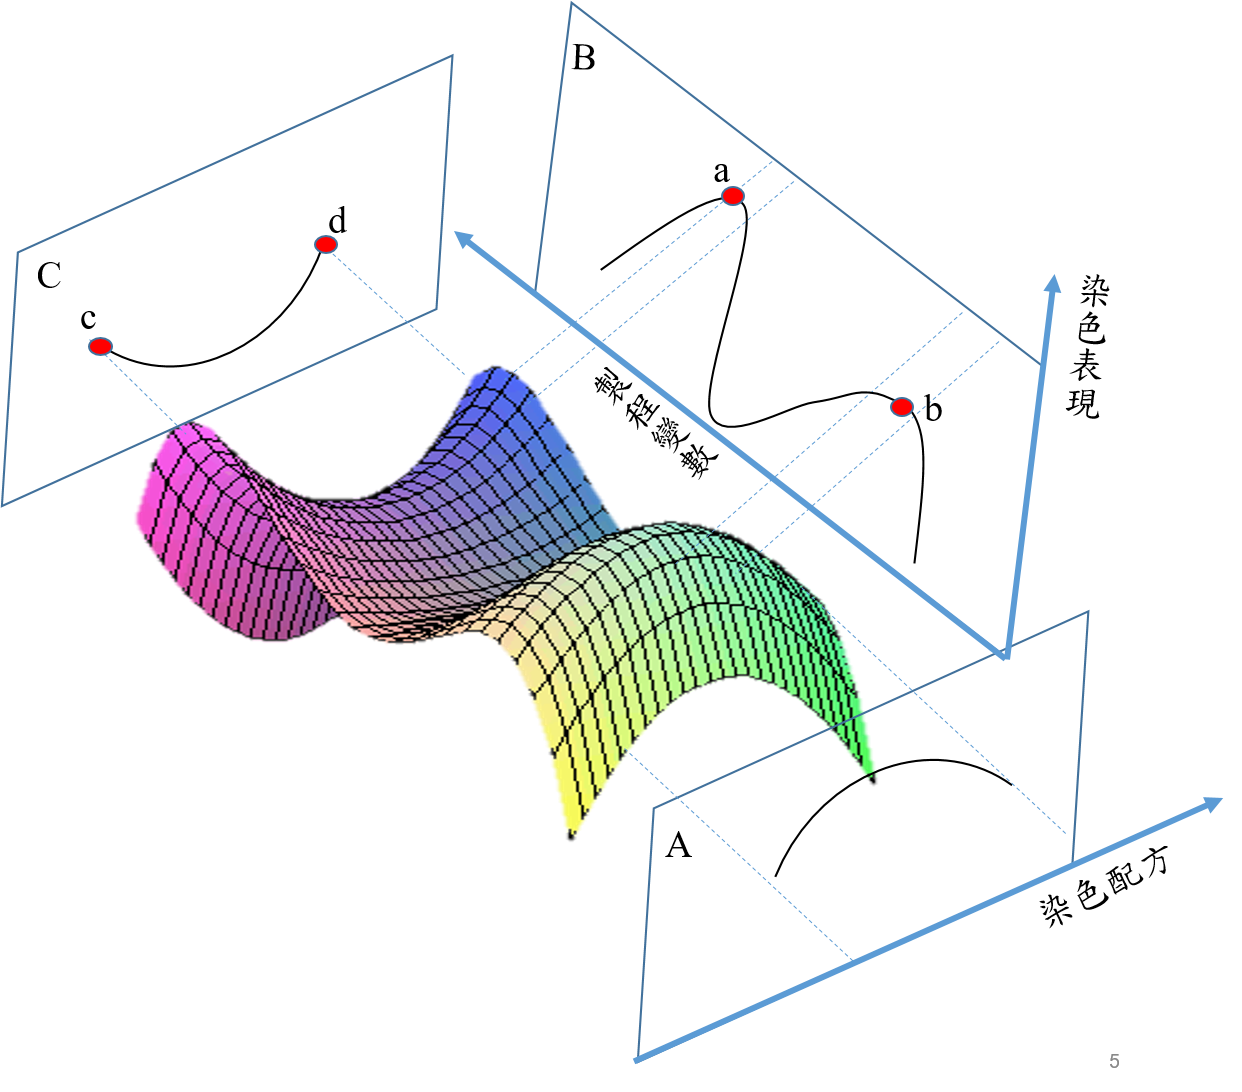
\includegraphics[width=12cm,height=10cm]{Graph/graph2.png}
\caption{染色配方和製程變數與染色表現的反應曲面}
\label{fig:graph2}
\end{figure}

由圖~\ref{fig:graph2}所示,如果單純的調整製程參數以降低成本,可能會造成已選定之染色配方不再是最佳選擇,或是單純的改變染色配方,也會使得已選定之製程參數並不是總成本最低的製程參數。本研究尋求總成本最低且較為穩健的製程變數及染色配方的組合,以降低染整現場的總成本。